%! TEX root = ../../../main.tex

\section{Handling Kubernetes Manifests}%
\label{sec:Handling_Kubernetes_Manifests}

\subsection{A Call for Better Manifest Management}%
\label{sub:A_Call_for_Better_Manifest_Management}
When configuring a microservice architecture to be deployed to a Kubernetes
Cluster, a lot of configuration files accrue. Each of these manifest files has
to be managed in some form. However, Kubernetes does not enforce any structure
upon how these files are stored and continuously managed. This lack of
standards makes it easy to get started with Kubernetes but can leave developers
stranded when working inside complex microservice architectures. In addition,
the microservice chapter (\ref{sub:Microservices}) already stated that
microservices are often developed in specialised teams. Thus, without any
management standard enforced by Kubernetes each microservice team can
theoretically define its own practises best fitting their preferences. This
might be tolerable inside a microservice team. However with respect to the
overall microservice architecture, different standards for managing Kubernetes
manifests make it harder for developers to understand the deployment structure
of their colleagues' microservices. Furthermore, with a common manifest
management standard every microservice can be set up the same way to be
deployed using a \ac{CI}/\ac{CD} system. Lastly, when needing support from an
external infrastructure operations team, a common manifest standard helps all
involved parties to exchange information faster and with less friction.

\subsection{Development}%
\label{sub:Development}
Chapter~\ref{ssub:Concepts} introduced a multitude of Kubernetes concepts that
will be referenced throughout this chapter. In addition,
chapter~\ref{ssub:Manifests} has shown that all infrastructure configurations of
Kubernetes are stored inside a YAML-based manifest file. This chapter will
build upon the knowledge from primarily these two chapters and try to develop
the best possible way to manage Kubernetes manifests in a microservice project.
Furthermore, the information presented in chapter~\ref{sub:Microservices} are
useful to understand the arguments presented in this chapter.

First, this section will show a \textit{naive} approach to continuously
deploying a microservice architecture to Kubernetes. Based on the problems
collected during this process, a better approach to manifest handling will be
derived. The whole process will be performed on the example of a specific
microservice architecture. The exemplary architecture contains a frontend, that
is being served by a NGINX web server, a user backend that manages the system's
users and an onboarding service that creates new users in the user backend. The
user and onboarding backend each have a separate non-relational MongoDB
database. Finally, the service adapter is responsible for resolving information
on an external application. For this purpose the service adapter also needs
access to the user's information. The whole infrastructure and the connections
between its microservices are also portrayed in figure~\ref{fig:dsp_excerpt}.

\begin{figure}[H]
\begin{center}
  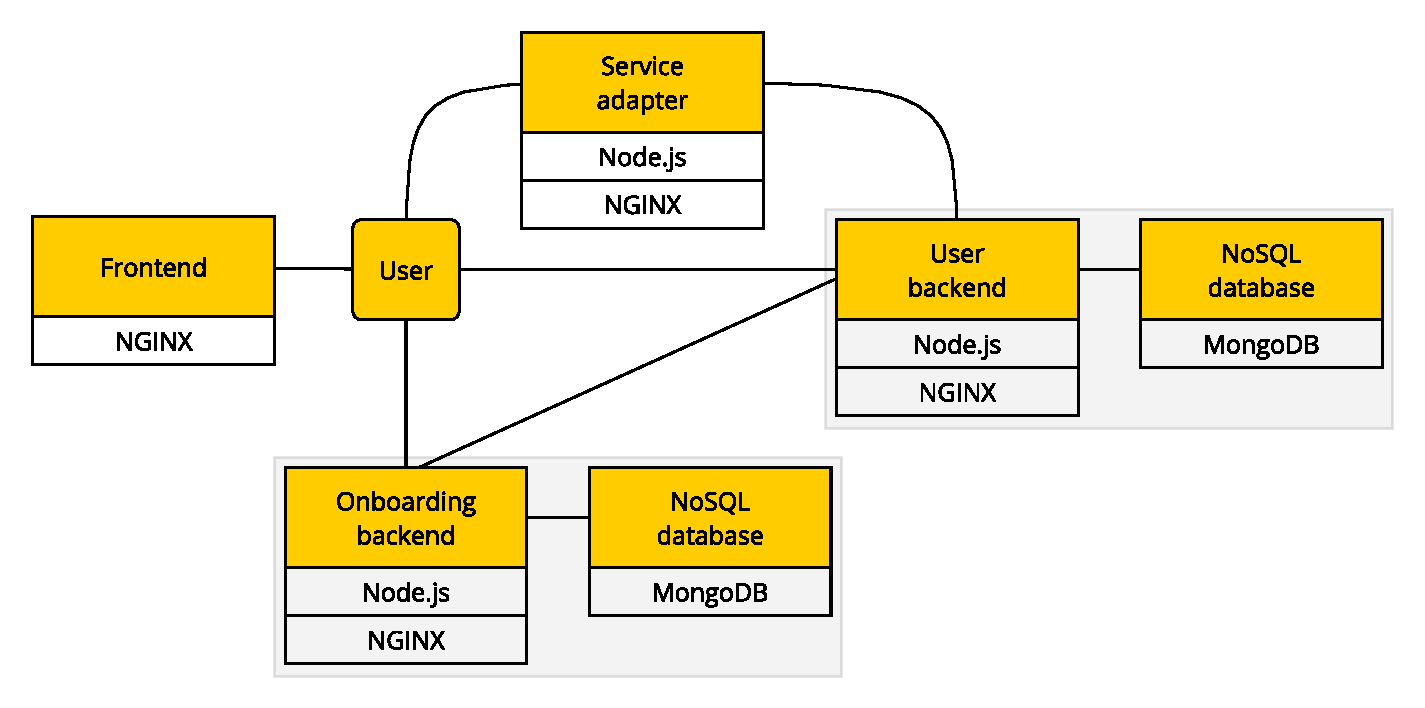
\includegraphics[scale=0.7]{images/figures/dspIT_excerpt.pdf}
\end{center}
\caption{The examplary $\mu$App microservice architecture containing three
backends and one frontend service.}%
\label{fig:dsp_excerpt}
\end{figure}

Throughout this chapter, this architecture will be referred to as
\textit{$\mu$App}. Even though the continuous deployment process will be
performed based on this software, $\mu$App is only an example for a
microservice architecture that can easily be exchanged with any other
microservice architecture.

\subsubsection{Deploying to Kubernetes: The Naive Way}%
\label{ssub:Deploying_to_Kubernetes_The_Naive_Way}

The first requirement for continuously integrating a software is that it is
tracked in a \ac{VCS}. In the case of $\mu$App, each service is managed in a
separate Git repository. Thus, each microservice has its own build and
deployment pipeline. When changes are pushed to the \texttt{master} branch, a
build pipeline is triggered.

\begin{listing}[H]
  \begin{minted}{YAML}
trigger:
- master
  \end{minted}
  \caption{Trigger definition for Microsoft Azure DevOps using the YAML-based syntax.}%
  \label{listing:master_trigger}
\end{listing}

Only pull requests can modify the data stored on the \texttt{master} branch.
This is achieved by using a YAML-based trigger definition as shown in
listing~\ref{listing:master_trigger}. Development work happens on independent
feature branches. After a feature is completed, the changes are merged into the
\texttt{development} branch where they reside until a pull request integrates
the changes into the \texttt{master} branch. Hence, only fully developed
features are build using the \ac{CI} pipeline and deployed using the \ac{CD}
process.

$\mu$App executes its \ac{CI} and \ac{CD} pipeline on the Microsoft Azure
DevOps service. As discussed in chapter~\ref{ssub:Continuous_Integration}, the
\ac{CI} process tests and builds the source code and constructs a Docker
container image. The image is then pushed to a central image repository. The
process is divided into multiple stages. The first stage is responsible for
building and testing $\mu$App whereas the second stage deploys the application
to Kubernetes. At this point, the \ac{CI} pipeline is completed and a
deployment is automatically triggered. This section will not focus any further
on the microservices' \ac{CI} process, as the interest is primarily aimed at
the procedure of continuously deploying a complete microservice architecture.

The overall deployment goal is to run $\mu$App on Kubernetes. Thus, its
microservices need a number of configuration objects to be either created or
updated in the cluster. Each service has one configuration file that is stored
in a separate \texttt{architecture} repository. Therefore a microservice's code
and its deployment manifests are fully isolated. Each manifest file holds all
the microservice's Kubernetes objects, e.g.\ Deployments, Services or
StatefulSets.  This is also the point where a distinction between microservices
that rely on a databases and microservice that do not have this dependency has
to be made. All services with an additional database component, e.g.\
$\mu$App's onboarding backend, have the Kubernetes objects that are needed to
deploy the database stored in a separate manifest file. Thus, in the case of
$\mu$App, the frontend and service adapter have one manifest file. On the other
hand, the onboarding and user backend have two manifest files; one for the
microservice's main Kubernetes objects and one for the microservice's database
Kubernetes objects.  This way, a clear separation of concerns is achieved.

When deploying a microservice, the pipeline reads the service's Kubernetes
manifest and deploys it to the cluster using Kubernetes' \texttt{kubectl}
utility. The service's database manifest however is not touched. Databases are
deployed by hand and independent from the \ac{CD} pipeline. Thus whenever a new
microservice is deployed, the service's database has to be deployed by hand
first. This can lead to situations in which the service can not be
automatically deployed because a required database component needs to be set up
manually first.

\begin{figure}[H]
\begin{center}
  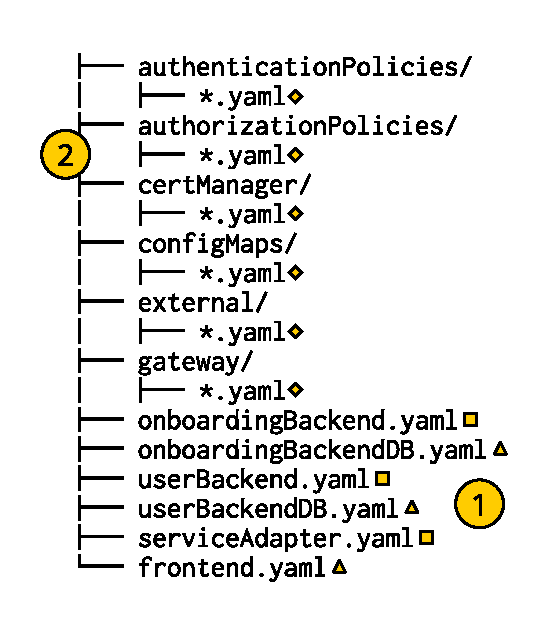
\includegraphics[scale=0.8]{images/figures/manifests_folder_naive.pdf}
\end{center}
\caption{Visualised folder structure of the \texttt{architecture} repository
holding $\mu$Apps' Kubernetes manifests.}%
\label{fig:manifests_folder_naive}
\end{figure}

\todo{Adapt a common spelling for \texttt{visualise} throughout the thesis.}

Figure~\ref{fig:manifests_folder_naive} visualises the folder structure that
holds $\mu$App's Kubernetes manifets. As already pointed out, all manifest
files are stored in a separate \texttt{architecture} repository. The files in
figure~\ref{fig:manifests_folder_naive} next to \circled{1} are the manifests
of all the $\mu$App's services as they were introduced in
figure~\ref{fig:dsp_excerpt}. Additionally a set of configurations are defined
next to \circled{2}. These files are stored in distinct directories and hold
configurations of authentication and authorization policies, \ac{HTTPS}
certificates, configuration maps, outgoing traffic rules and the Ingress
gatway. This way, the infrastructure configuration is entirely detached from
microservices' one.

When deploying $\mu$App from scratch, a three step process must be completed.
First, the underlying infrastructure needs to be set up. This includes all
network and storage settings. Then the microservices' databases have to be set
up. At last the actual application manifests are applied to the Kubernetes
cluster. The process requires active monitoring of the Kubernetes objects to
make sure that all configurations of a step are fully applied before starting
the next step.

Due to the file structure of the application's manifest files, it is not
possible to apply all manifests of one stage. Thus when mapping the deployment
steps to the manifest files, in stage one, the files marked with a
\inlineDiamond{} are applied. The database manifests files marked with
\inlineRectangle{} are then applied. They create the services' databases.
Lastly, the files marked with \inlineTriangle{} are applied. After this step is
completed, $\mu$App is fully deployed from scratch. All markings mentioned in
this section refer to figure~\ref{fig:manifests_folder_naive}.

This concludes the \textit{naive} deployment approach for $\mu$App. The
approach reveals a number of issues that need to be solved in order to have a
fully autonomous continuous deployment process. For the purpose of
traceability, these issues are labelled $I_1$ to $I_n$. The issues include:

\begin{itemize}
  \item \textit{$I_1$}: A \ac{CI} process is only started when changes are
    merged from the independent \texttt{feature} branches to the
    \texttt{master} branch. Thus the rule that software should be built every
    time a new change is present in the \ac{VCS} is not met.
  \item \textit{$I_2$}: When deploying $\mu$App from scratch, the deployment is
    comprised of three steps that need to be executed by hand.
  \item \textit{$I_3$}: The deployment of the actual microservice and its
    database is decoupled and they thus are executed independently from one
    another.
  \item \textit{$I_4$}: A microservice's database has to be deployed first to
    guarantee its available once the actual microservice using that database is
    deployed.
  \item \textit{$I_5$}: A microservice's manifest files are managed
    independently from the services actual source code. This gap means that two
    distinct lifecycles must be managed.
\end{itemize}

Despite these issues that already reveal themselves when inspecting the
deployment model statically, an additional issue could be observed when using
the model in practise:

\begin{itemize}
  \item \textit{$I_6$}: The second a microservice looses the connection to its
    database, it becomes dead and unusable. The only way to recover it from
    this state is to kill the pods hosting the application, making sure that
    the database is available again and than restarting the microservice's pod.
\end{itemize}

\subsubsection{Deploying to Kubernetes: An Improved Approach}%
\label{ssub:Deploying_to_Kubernetes_An_Improved_Approach}

This section will try to develop an improved approach to managing Kubernetes
manifests in a microservice project that is continuously deployed. It will base
the development on the same architecture that was introduced in
figure~\ref{fig:dsp_excerpt} and the findings of the previous
section~\ref{ssub:Deploying_to_Kubernetes_The_Naive_Way}. The overall goal is
to solve the issues identified by the naive deployment approach explored
previously. With the help of these solutions, the problem domain's questions of
how Kubernetes manifests should be managed and deployed in a continuously
deployed microservice architecture can be answered.

To get started, issue $I_6$ does not only relate to continuously deployed
microservices but rather to any service that is deployed to a Kubernetes
cluster. As pointed out in chapter~\ref{sub:Kubernetes} it is in the service's
nature which are executed on Kubernetes to be constantly created, killed and
moved between hosts. Thus any service that wants to withstand such harsh
conditions has to be resilient when dealing with dropping connections. This is
not only limited to database connections. However databases can be used
representationally for this issue.

Issue $I_6$ can be solved on two layers. Either Kubernetes deals with a
service's connection or the service itself takes on this task. To decide which
layer fits the situation at hand best, it has to be distinguished between
applications which enter a state they can not recover from when their
connection to a database is dropped and applications which can recover from
such a state. In cases where the application can not recover itself from such a
state, it either has to be customized to be able recover itself or Kubernetes
is forced to deal with the situation. In case the application can not adapt
such functionality, a Kubernetes liveness probe can be used to determine
whether the application is still running functionally. The liveness probe
executes a command inside the application's container, \ac{HTTP} request or
\ac{TCP} call. If the probe reports that the service is not alive any more,
Kubernetes automatically kills the application's container and restarts it.
This way, the application does not have to deal with such situations itself and
behaviour that leads the application to crash can be intercepted without the
application having to adapt \autocite{AuthorsConfigureLivenessReadiness2019}.
The application's developers only have to implement an interface for Kubernetes
to determine the application's status. In the case of microservices which offer
a \ac{REST} interface over \ac{HTTP} a simple \texttt{/health} endpoint would
suffice. Though implementing a simple interface might seem like test best
solution for all types of applications, one important notice has to be made. It
must be assessed whether the application's full start-up when restarting its
containers is too resource-heavy. An application which simply hosts static
files like $\mu$App's frontend service restarts within seconds whereas
$\mu$App's service adapter which rebuilds its cache from scratch every time it
starts takes a long time and many resources to perform a full restart.

\begin{listing}[H]
  \begin{minted}{text}
HTTP/1.1 200 OK
content-type: application/json; charset=utf-8
content-length: 18
connection: close

{"status":"alive"}
  \end{minted}
  \caption[A REST health endpoint stating that the service is alive.]{A
  \ac{REST} health endpoint stating that the service is alive.}%
  \label{listing:health_endpoint_http}
\end{listing}

Listing~\ref{listing:health_endpoint_http} shows an exemplary \ac{HTTP}
response of a \ac{REST} \ac{API} that states that the service is running
without problems. Hence, issue $I_6$ can be solved with relatively little
implementation work when using Kubernetes' built-in features.

In the naive deployment approach only commits to the \texttt{master} branch
would be built and deployed. This however conflicts with the \ac{CI} guidelines
as outlined by chapter~\ref{ssub:Continuous_Integration}. To build all branches
of a project, the same pipeline definition file can be used. The trigger
definition as shown in in listing~\ref{listing:master_trigger} has to be
dropped. When dropped, Azure DevOps builds all changes across all branches of a
imply dropping the trigger definition would however create a new problem. Due
to the fact that the pipeline was previously only run when stable changes were
pushed to the master branch, all changes would be automatically deployed. By
just dropping the trigger definition all changes from all branches would be
built, tested, packed into a Docker image and pushed to a central container
image repository. However a pipeline that is being triggered from changes in a
branch other than the \texttt{master} branch should only be built and tested
thus only undergoing the pipeline's \ac{CI} part. To implement such a
behaviour, pipeline conditions can be used. Conditions can be applied to both
jobs and stages. As $\mu$App's pipeline is made up of two stages, the first
building and testing the application and the second deploying it to Kubernetes,
only the second stage has to protected by a condition.

\begin{listing}[H]
  \begin{minted}{YAML}
stages:
- stage: Deploy
  displayName: Deploy to Kubernetes
  dependsOn: Build
  condition: and(succeeded(), eq(variables['Build.SourceBranch'],
                 'refs/heads/master'))
  jobs:
    - ...
  \end{minted}
  \caption{A Microsoft Azure DevOps pipeline stage being protected by a
  condition (condition taken from \autocite{MicrosoftConditions2019}).}%
  \label{listing:pipeline_condition}
\end{listing}

Listing~\ref{listing:pipeline_condition} displays how a condition can be set
for a stage that handles the deployment of $\mu$App. If no condition is set for
a stage, Azure DevOps automatically applies the \texttt{succeeded()}
expression. Thus, by default to execute a stage, the previous stage had to be
successful. The \texttt{and} expression in line five of
listing~\ref{listing:pipeline_condition} only return \texttt{true} if both its
parameters return \texttt{true} individually. Thus, the \texttt{Deploy} stage
is only computed if the previous stage performed successfully and the build is
triggered by a change in the \texttt{master} branch. Hence, the same Azure
DevOps pipeline can be used for both releasing stable as well as building and
testing branches that are under active development. This concludes the solution
of issue $I_1$.

Up next, issue $I_4$ can be partially answered using the same technique already
presented as the solution to issue $I_6$. A microservice that depends on a
database for its start up can use Kubernetes's built-in liveness probe to
determine if the application crashed due to a missing database component which
has not started yet. In case a liveness probe is not suitable for the
application at hand, e.g.\ due to a resource consuming start up process, the
application has to be fitted with a more rigid database connection process.

\begin{figure}[H]
  \hspace*{\fill}%
  \subfloat[Using Kubernete's liveness probe to handle a failed database connection during a microservice's start up. \label{subfig:database_connection_probe}]{%
    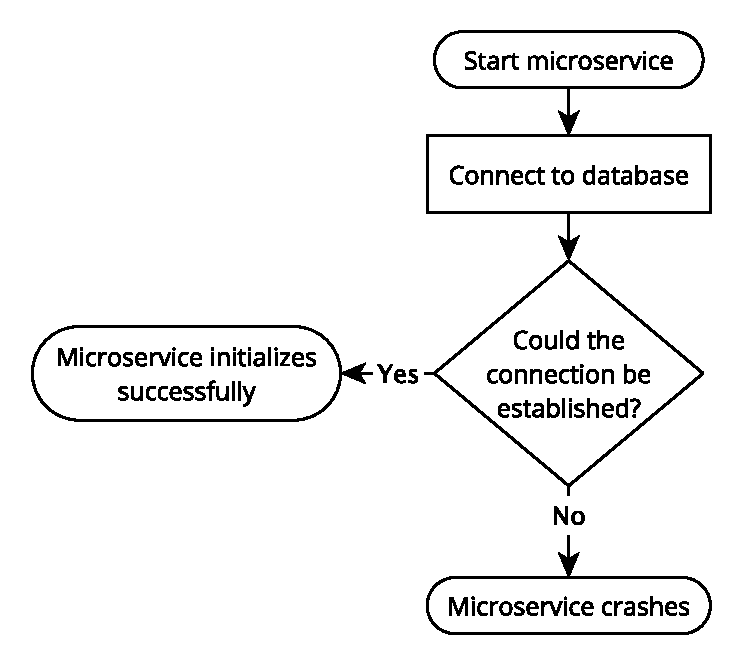
\includegraphics[scale=0.55]{images/figures/database_connection_probe.pdf}
  }
  \qquad
  \subfloat[Implementing a timeout to handle a failed database connection during microservice's start up. \label{subfig:database_connection_timeout}]{%
    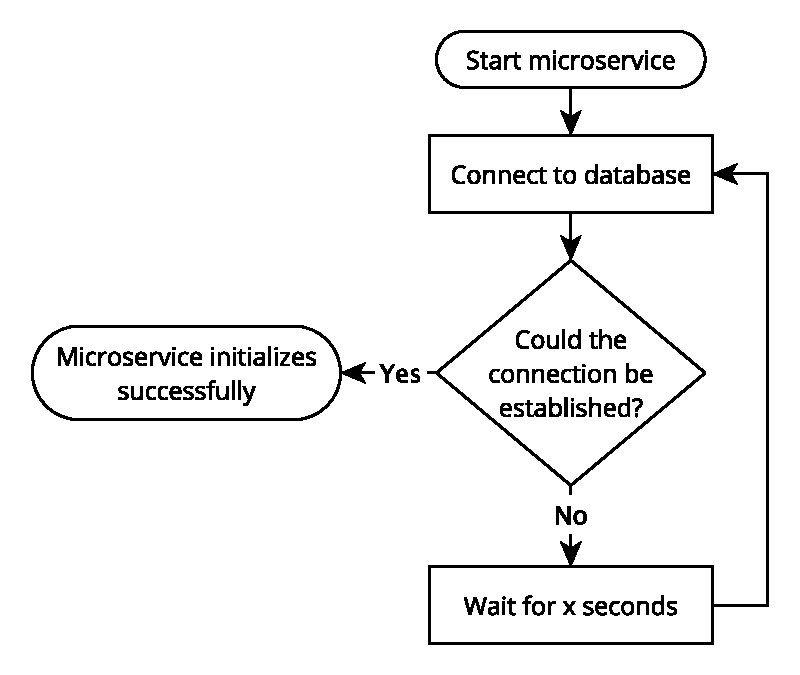
\includegraphics[scale=0.55]{images/figures/database_connection_timeout.pdf}
  }
  \hspace*{\fill}%

  \caption{Two ways to handle a failed database connection during a microservice's start up.}%
  \label{fig:database_connection_start_up}
\end{figure}

Figure~\ref{subfig:database_connection_probe} shows how an application can
handle a failed database connection using Kubernete's liveness probe. When
starting the service, it tries to establish a connection to its external
database component. If this fails, the application crashes and enters a state
from which it can not recover without Kubernete's help. Kubernetes detects the
service's state and restarts its container. If a database is available on the
service's second start up, its launch can be considered successful. This cycle
is repeated as long as the external database component is not ready to receive
connection.

On the other hand, figure~\ref{subfig:database_connection_timeout} shows a more
robust solution that does not depend on Kubernete's liveness probe. Instead of
letting the application enter a state from which it cannot recover from again,
a timeout can be implemented in the microservice. After a database connection
establishment failed, the application waits $x$ seconds and tries to connect
again. This cycle is repeated until a successful connection can be established.

Using one of these two approaches, issue $I_4$ can be considered solved.

Next, the issues $I_2$, $_3$ and $I_5$ can be dealt with collectively. Even if
their nature appears to be quite different, a well though \textit{Kubernetes
manifest management} concept helps to solve them. The upcoming section will try
to formulate such a concept that defines in \textit{which place} and
\textit{which format} Kubernetes manifests should be stored. In addition this
concept will outline how these manifests are rolled out continuously and from
scratch. To understand the idea behind the concept, the basic knowledge of Helm
as outlined in chapter~\ref{sub:Helm} is required.

To recap, each component of $\mu$App is stored in a distinct tac{VCS}
repository. Nonetheless, The Kubernetes manifest needed to deploy $\mu$App are
managed in a completely different repository called \texttt{architecture}. As a
result, two separate lifecycle management processes are required to manage the
application's code and its manifest files. To overcome this, the services'
Kubernetes manifests are moved from the \texttt{architecture} repository to
their respective service's code repository. Hence, the two management processes
are no longer decoupled. Every time that code is modified in the services'
repository, the manifest files have to be updated too if architecture changes
are needed. Thus, a deployment manifest is always tagged to the latest commit
in a service's code repository. So far this solves issue $I_5$ and gives an
answer to the question in which place manifest files should be stored. Yet it
does not comprise a complete manifest management concept.

To achieve this, the Kubernetes package manager Helm can be utilized. Instead
of storing a service's manifests loosely next to the service's source code
files or in some arbitrary named directly in the service's \ac{VCS} repository,
each service gets it individual Helm chart. For each of $\mu$App's services, a
directory called \texttt{deployment} is created in the project's root folder.
Caused by Helm's naming requirements, the \texttt{deployment} directory houses
another directory bearing the name of the service. $\mu$App's frontend service
e.g.\ thus houses a \texttt{deployment/frontend} directory whereas the user
backend holds a \texttt{deployment/user-backend} folder structure.

\begin{figure}[H]
\begin{center}
  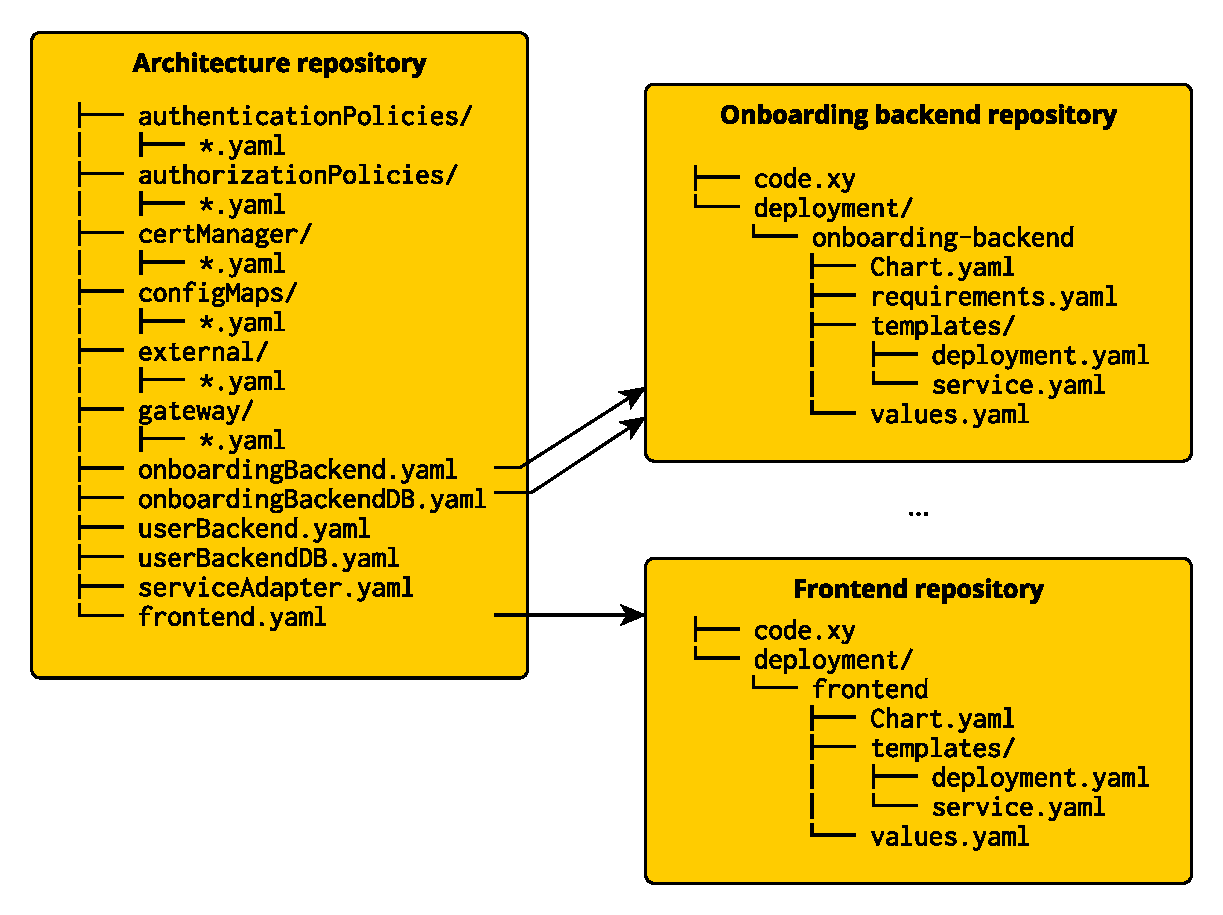
\includegraphics[scale=0.7]{images/figures/helmification_process.pdf}
\end{center}
\caption{The transition from a separate repository holding a service's
configuration to each microservice repository managing its respective
Kubernetes manifests.}%
\label{fig:helmification_process}
\end{figure}

Figure~\ref{fig:helmification_process} shows the process of transforming from a
central deployment manifest management to a decentralized management concept
using Helm. The figure visualizes the transformation process on the example of
$\mu$App's onboarding backend and frontend. The frontend which does not depend
on a database or any other external Kubernetes components does not have a
\texttt{requirements.yaml} file. Hence, Helm does not need to install any
additional software. On the contrary, the onboarding backend needs a database
component. Therefore, a \texttt{requirements.yaml} file is present in the newly
created Helm chart inside the onboarding backend's repository.

\begin{listing}[H]
  \begin{minted}{YAML}
dependencies:
  - name: mongodb-replicaset
    version: 3.9.6
    repository: https://kubernetes-charts.storage.googleapis.com/
  \end{minted}
  \caption{Helm's requirements file for $\mu$App's onboarding backend.}%
  \label{listing:onboarding_backend_requirements}
\end{listing}

It defines an external database component (\texttt{mongodb-replicaset}) as
shown in listing~\ref{listing:onboarding_backend_requirements} which is
automatically set up whenever the onboarding backend is deployed by Helm.
Therefore issue $I_3$ can be considered solved as well. The deployment process
of a service and its external dependencies, e.g.\ a database, is no longer
decoupled.  For this purpose the onboarding backend also creates a
\texttt{charts} directory which stores the service's packed dependencies. This
directory however is not listed in figure~\ref{fig:helmification_process}
because it does not need to exist in the \ac{VCS}. The folder is only created
on the machine deploying the microservice once the installation process is
triggered.

So far this approach already solves issue $I_5$. Managing a microservice's code
and its deployment information is no longer decoupled. This comprises a partial
manifest management concept answering the questions \textit{where} and in
\textit{which format} manifests are stored. Though it is now possible to deploy
each of $\mu$App's microservices using the respective Helm chart, the process
requires a number of manual inputs. Continuously releasing helmified
microservices is only limitedly possible. To enable a fully automatic and
continuous release process for helmified microservices, these problems have to
be addressed:

\begin{itemize}
  \item The Helm charts only live inside their respective microservice's
    \ac{VCS} repository in a non-built form. Hence, to deploy a service, the
    entire repository has to be fetched in order to read the chart information.
  \item To deploy $\mu$App's full microservice architecture, each service has
    to be deployed manually one by one. No mechanism exists yet to deploy the
    complete microservice architecture at once.
  \item Each time the microservice's code is updated, the \texttt{appVersion}
    property inside the service's \texttt{Chart.yaml} has to be updated to
    reflect the builds current version. So far this is a manual process. At the
    same time the chart's \texttt{version} property has to be bumped so that a
    chart's version (e.g.\ 1.2.1) never points to more than one app version
    (e.g.\ 3.4.1 and 3.4.2).
\end{itemize}

Rather than just storing the Helm charts inside the service's repository, a
built version of the chart should be saved to some chart repository. The
\texttt{mongodb-replicaset } chart referenced in
listing~\ref{listing:onboarding_backend_requirements} e.g.\ is hosted as part
of Helm's official and publicly accessible \texttt{stable} repository. However
not every chart should be accessible to the general public.  With $\mu$App the
architecture is comprised of a set of internal services which deployment
information should not be publicly accessible. In such cases, a private
repository can host the Helm charts.

In general, a chart repository is a simple webserver which serves an
\texttt{index.yaml} file that is fetched and parsed by a Helm client. The file
holds references to all charts hosted by the repository including their name,
version number and packaged chart file. One solution implementing such a
functionality is called \texttt{ChartMuseum}. Not only does ChartMuseum manage
and store charts, it also includes a \ac{REST} \ac{API} which allows to add new
charts, update existing ones and deletes old ones. For the purpose of hosting
$\mu$App's microservice charts, an instance of CartMuseum is deployed to
Kubernetes and made accessible from outside Kubernetes. Additionally,
ChartMuseum allows to set an authentication method for both fetching charts as
well as publishing them. This feature is also enabled for this instance of
ChartMuseum to shield it from unauthorized access. For the purpose of
simplicity, only the \textit{basic} \ac{HTTP} is used though other mechanism
are supported.

Now every time a Helm chart is updated, e.g.\ because the \texttt{appVersion}
attribute is bumped or a deployment setting is modified, this change no longer
just lives inside the service's repository. The chart is also packaged and
pushed to the internally hosted ChartMuseum instance. Then when this service
should be deployed to Kubernetes, the Helm client running the deployment can
add the ChartMuseum chart repository, fetch the chart without fetching the
service's code and deploy it to Kubernetes.

To recap, it is the overall goal to deploy microservices \textit{continuously}.
Thus, this manifest management concept is not sufficient, yet. To become fully
sufficient, an element of automation has to be reintroduced. Instead of
updating, packaging and publishing a Helm chart by hand each time a service's
code base is updated, a \ac{CI} solution can take on this job. Again, Azure
DevOps is used as a reference for a \ac{CI} solution in the upcoming examples.

\begin{listing}[H]
  \begin{minted}[escapeinside=**]{YAML}
- job: Create_Chart
  dependsOn: Build
  steps:
  - task: HelmInstaller@1
    inputs:
      helmVersionToInstall: 'latest'
  - script: |
      sed -i "s/version: \"latest\"/version: \"$BUILD_BUILDNUMBER\"/g" \
      deployment/*\textbf{service-name}*/values.yaml
  - task: HelmDeploy@0
    inputs:
      command: 'package'
      chartPath: *\textquotesingle*$(System.DefaultWorkingDirectory)/deployment/*\textbf{service-name}\textquotesingle*
      chartVersion: '1.0.0+$(Build.BuildNumber)'
      arguments: '--app-version 1.0.0+$(Build.BuildNumber)'
  - script: |
      curl --user username:password \
      --data-binary "@$(Build.ArtifactStagingDirectory)/ \
        *\textbf{service-name}*-1.0.0+$(Build.BuildNumber).tgz" \
        https://domain.local/internal/chartmuseum/api/charts
  \end{minted}
  \caption{An Azure DevOps job which installs the Helm client, sets the
  service's container image to the one produced by the build, packages the
  chart and pushes the chart to a ChartMuseum instance.}%
  \label{listing:azure_devops_build_chart_job}
\end{listing}

To continuously produce an updated Helm chart when (code) changes are pushed to
a service's repository, the Helm client has to be installed first (line 4-6,
listing~\ref{listing:azure_devops_build_chart_job}). As already pointed out,
container images produced by the \ac{CI} system are tagged with the current
build number. Each version of a service's Helm chart should always point
deterministically to a specific container image version and not use the
\texttt{latest}. This avoids situations in which a Helm chart is deployed once
and e.g.\ installs application version 1.2.0 and one year later installs
application version 3.1.0 because the \texttt{latest} tag moved along as new
versions of the software are created.

\begin{listing}[H]
  \begin{minted}[escapeinside=**]{YAML}
container:
  name: *\textbf{service-name}*
  version: "latest"
  \end{minted}
  \caption{A service's \texttt{values.yaml} Helm file specifying a container
  image name and version number.}%
  \label{listing:helm_values_ci_image_version}
\end{listing}

Lines 7-9 of listing~\ref{listing:azure_devops_build_chart_job} show how the
current build number can be injected into a service's \texttt{values.yaml}
file. For reference, an exemplary values file is shown in
listing~\ref{listing:helm_values_ci_image_version}. During each build, the
\ac{CI} system searches for the string \texttt{version:``
latest''} and replaces it with
\texttt{version:``\textbf{build-number}''}. The result is
then written in the service's \texttt{values.yaml} file. These changes only
live inside the build pipeline and are not persistently written into the
\ac{VCS} system.

In the next step (shown in line 10-15 of
listing~\ref{listing:azure_devops_build_chart_job}) a built-in Azure DevOps
tasks is used to package the service's chart. In the process, the chart's
version number is bumped to the SemVer version number
\texttt{1.0.0+\textbf{build-number}}. Additionally, the chart's
\texttt{appVersion} property is updated to reflect the current build number.
These new version numbers are only visible inside the packaged Helm chart. They
are not written into the unpackaged \texttt{Chart.yaml} file as there is no
need to transfer the changes to the service's repository.

At last, line 16-20 of listing~\ref{listing:azure_devops_build_chart_job} show
how the newly packaged chart is uploaded to the internal ChartMuseum instance.
ChartMuseum's username and password combination is supplied to authenticate the
\texttt{curl} request. At this point, the internal chart repository hosted by
ChartMuseum serves the newly created Helm chart which specifically points to
the newest built container image and which is versioned based on the build's
number.

\begin{figure}[H]
\begin{center}
  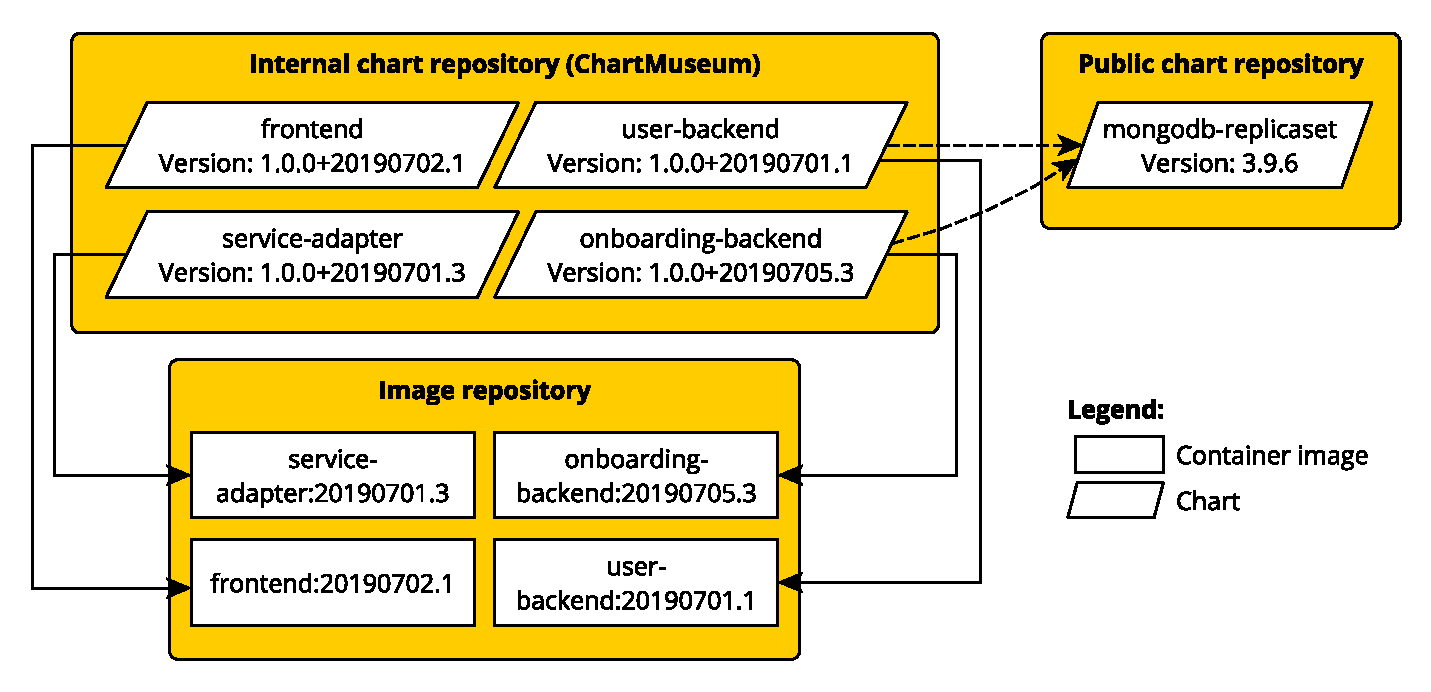
\includegraphics[scale=0.6]{images/figures/chart_to_image_mapping.pdf}
\end{center}
\caption{A visual representation of the storage locations, version numbers and
image dependencies of $\mu$App's Helm charts.}%
\label{fig:chart_to_image_mapping}
\end{figure}

Figure~\ref{fig:chart_to_image_mapping} shows the mappings from a Helm chart to
the corresponding referenced container image that are created by the \ac{CI}
system as outlined in listing~\ref{listing:azure_devops_build_chart_job}. Each
chart receives a unique version number based on the SemVer
\texttt{MAJOR.MINOR.PATCH+\textbf{build-number}} scheme. The corresponding
Docker images use a similar tag while dropping the \texttt{MAJOR.MINOR.PATCH}
part. In addition, the figure shows that both the user backend as well as the
onboarding backend depend on an publicly hosted MongoDB Helm chart.

Up to this point the creation of individual Helm charts for each service is
fully automated using a \ac{CI} solution like Azure DevOps. However, no
automated continuous deployment process exists yet. One option would be to use
the Helm utility to upgrade the respective chart in Kubernetes within a
service's Azure DevOps pipeline. This would automate the second and third step
of the last issue $I_2$ but leave the first step to be executed by hand. To
recap, the first deployment step referenced in in issue $I_3$ is a set up of
the underlying infrastructure. Step two sets up a service's external
dependencies and lastly step three deploys the service's actual application.
How can the now existing automation process of step two and three be combined
with step one to form a fully autonomous manifest management and deployment
concept for a microservice architecture? After all, it is not always possible
to assign infrastructure configurations to a distinct service. Kubernetes
StorageClass definitions e.g.\ might be relevant to all microservice of a
application. 

\begin{figure}[H]
\begin{center}
  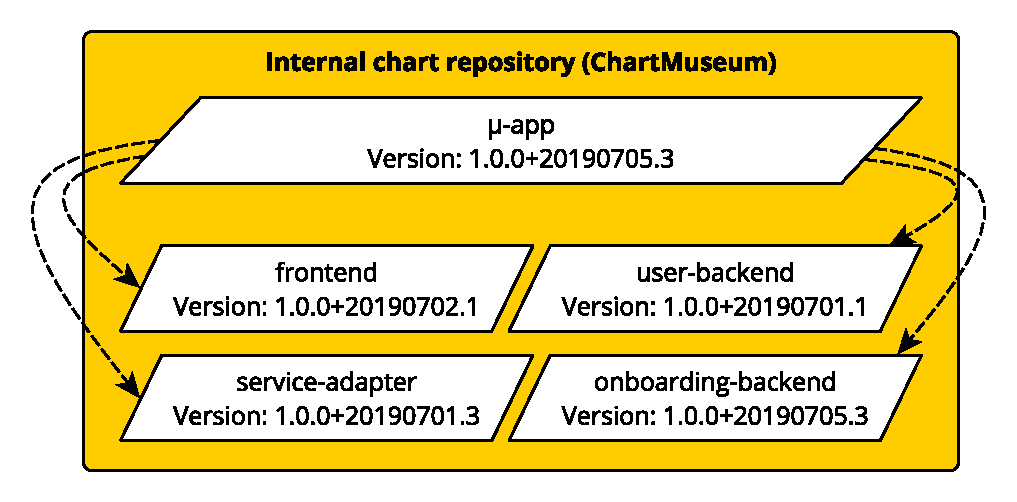
\includegraphics[scale=0.7]{images/figures/master_chart.pdf}
\end{center}
\caption{A master chart which defines a microservice architecture's individual
services as dependencies and which is continuously versioned.}%
\label{fig:master_chart}
\end{figure}
